\documentclass[compress]{beamer}
\usepackage[latin1]{inputenc}
\usepackage{default}

\setbeamercovered{transparent}
\setbeamertemplate{navigation symbols}{} % remove navigation symbols


% \useoutertheme[subsection=false]{smoothbars} % Beamer Outer Theme
% \useinnertheme{rectangles}

  \usetheme{Warsaw}
% \usetheme{default}
% \usetheme{Boadilla}
% \usetheme{Madrid}
% \usetheme{Montpellier}
% \usetheme{Copenhagen}
% \usetheme{Goettingen}
% \usetheme{Hannover}
% \usetheme{Berkeley}
% \usetheme{Ilmenau}

% \usecolortheme{seahorse}
% \usecolortheme{beaver}
% \usecolortheme{rose}
% \usecolortheme{beetle}
% \usecolortheme{crane}
% \usecolortheme{default}
% \usecolortheme{dolphin}

% \setbeamercolor{block title}{fg=black,bg=gray!40}
% \setbeamercolor{block body}{fg=black,bg=gray!10}
% \setbeamercolor{block title alerted}{fg=red,bg=green!40}
% \setbeamercolor{block title example}{fg=black,bg=green!20}
% \setbeamercolor{block body example}{fg=black,bg=green!5}
% \setbeamerfont{block title}{series=\bfseries}


\title[Online Handwriting Recognition] % (optional, use only with long paper titles)
{Reconocimiento de Escritura Manuscrita \\
\footnotesize{\textbf{\textit{(Online Handwriting Recognition)}}}
}

\author[Tesina de Grado - Pablo Speciale]
{\textsc{Pablo Speciale}}

\date[Septiembre 2011] % (optional, should be abbreviation of conference name)
{\textbf{Tesina de Grado} \\ \tiny{\textit{(Septiembre 2011)}}}
% - Either use conference name or its abbreviation.
% - Not really informative to the audience, more for people (including
%   yourself) who are reading the slides online

% \author[Tesina - Pablo Speciale]
% {Pablo Speciale \and Juan Carlos G�mez\inst{1} \and Pablo Granitto\inst{2}}
% - Give the names in the same order as the appear in the paper.
% - Use the \inst{?} command only if the authors have different
%   affiliation.

% \institute
% {
% \inst{1}%
%     Procesamiento de Se�ales Multimedia, CIFASIS\\
%     gomez@cifasis-conicet.gov.ar
% \and
% \inst{2}%
%     Aprendizaje Automatizado y Aplicaciones, CIFASIS \\
%     granitto@cifasis-conicet.gov.ar
% }
% - Use the \inst command only if there are several affiliations.
% - Keep it simple, no one is interested in your street address.



% Structuring a talk is a difficult task and the following structure
% may not be suitable. Here are some rules that apply for this
% solution:

% - Exactly two or three sections (other than the summary).
% - At *most* three subsections per section.
% - Talk about 30s to 2min per frame. So there should be between about
%   15 and 30 frames, all told.

% - A conference audience is likely to know very little of what you
%   are going to talk about. So *simplify*!
% - In a 20min talk, getting the main ideas across is hard
%   enough. Leave out details, even if it means being less precise than
%   you think necessary.
% - If you omit details that are vital to the proof/implementation,
%   just say so once. Everybody will be happy with that.



\begin{document}

% \begin{frame}
%   \titlepage
% %     \begin{center}
% %     \includegraphics[scale=0.16]{cifasislogo}
% %     \end{center}
% \end{frame}

\section{Introducci\'on}

\subsection{S\'intesis de Texturas}

\begin{frame}[plain]
\titlepage
\vspace*{-1.25 cm}
\begin{center}
    
\includegraphics[scale=0.025]{../imagen/logo_fceia.pdf}
    \hspace*{5cm}
    
\includegraphics[scale=0.156]{../imagen/logo_unr.pdf}
\end{center}
\vspace*{-0.5 cm}
\begin{center}
\tiny{\textit{Lic. en Cs. de la Computaci�n \\
Facultad de Ciencias Exactas, Ingenier�a y Agrimensura \\
Universidad Nacional de Rosario}}
\end{center}

\vspace*{0.65 cm}
\begin{footnotesize}
\textbf{Director}: Dr. Juan Carlos Gomez\footnote{\textit{\tiny{Procesamiento de Se�ales Multimedia}, CIFASIS}} \\
\textbf{Co-director}:  Dr. Pablo Granitto\footnote{\textit{\tiny{Aprendizaje Automatizado y Aplicaciones}, CIFASIS}}
\end{footnotesize}
\end{frame}


\begin{frame}[plain]
\frametitle{�ndice}
\scriptsize % Para r e d u c i r e l tama \~ no de l e t r a
\tableofcontents
\end{frame}


\begin{frame}
%     \begin{Example}
        \begin{center}
        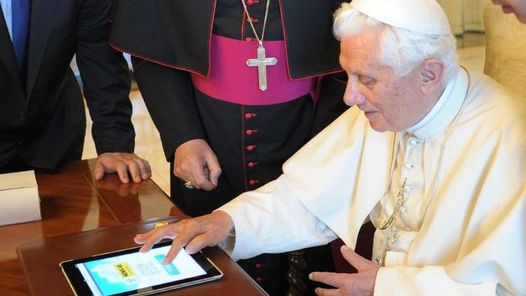
\includegraphics[scale=0.5]{papa.jpg}
        \end{center}
%     \end{Example}
\end{frame}


\begin{frame}[<+->]
\frametitle{There Is No Largest Prime Number}
\framesubtitle{The proof uses \textit{reductio ad absurdum}.}
    \begin{theorem}
    There is no largest prime number.
    \end{theorem}
    \begin{proof}
    \begin{enumerate}
    \item<1-| alert@1> Suppose $p$ were the largest prime number.
    \item<2-| alert@2> Let $q$ be the product of the first $p$ numbers.
    \item<3-| alert@3> Then $q+1$ is not divisible by any of them.
    \item<1-> Thus $q+1$ is also prime and greater than $p$.\qedhere
    \end{enumerate}
    \end{proof}

    \begin{block}{Block title}
        \begin{itemize}
        \item<2-> \alt<2>{\color{blue} Everything}{\color{black} Everything}
        \item<2-> \alt<3>{\color{blue} that has}{that has}
        \item<2-> \alt<4>{\color{blue} beginning}{\color{red} beginning}
        \item<2-> \alt<5>{\color{blue} has end.}{\color{green} has end.}
        \end{itemize}
    \end{block}
\end{frame}


\begin{frame}
    \begin{block}{title}
        test \\
        a second line
    \end{block}
    \begin{block}{}
        test without title
    \end{block}
    \begin{alertblock}{title}
        test
    \end{alertblock}
    \begin{Example}
        test
    \end{Example}
\end{frame}


\end{document}
